\name{grlogsp}{draw a running log spectrum graph}{plotting graphs}

\begin{synopsis}
\item[grlogsp] [ --t ] [ --O $O$ ] [ --x $X$ ] [ --y $ymin$ ] [ --yy $YY$ ]
	       [ --yo $YO$ ] [ --p $P$ ] 
\item[\ ~~~~~~~~] [ --ln $LN$ ] [ --s $S$ ] [ --e $E$ ] [ --n $N$ ] [ --l $L$ ] 
\item[\ ~~~~~~~~] [ --c $comment1$ ] [ --c2 $comment2$ ] [ --c3 $comment3$ ]
		  [ {\em infile} ]
\end{synopsis}

\begin{qsection}{DESCRIPTION}
The command {\em grlogsp} reads data from the standard input
in float format, evaluates its running log spectrum, and
generates an output file which includes the sequence of commands
so that it can be plotted(FP5301 protocol).
This command can be used in connection with commands such as ``xgr''.
\par
Actually, it uses {\em fig} and {\em fdrw} commands through a
shell script.
\end{qsection}

\begin{options}
	\argm{t}{}{transpose x and y axes}{FALSE}
	\argm{O}{O}{origin of graph\\
		      \begin{minipage}{4cm}
		      \begin{tabular}{ccc}
			1 & ( 25,$YO$) & [mm] \\
			2 & ( 60,$YO$) & [mm] \\
			3 & ( 95,$YO$) & [mm] \\
			4 & (130,$YO$) & [mm] \\
			5 & (165,$YO$) & [mm]
		      \end{tabular}\\\hspace*{\fill}
		      \end{minipage}
		      \begin{minipage}{4cm}
			    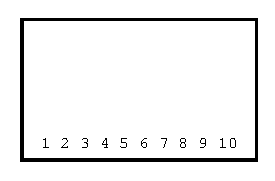
\includegraphics{fig/grlogsp-on.eps}
		      \end{minipage}\\\hspace*{\fill}\\
		    $(YO + 100 , X)$ [mm] if -t is specified.}{1}
	\argm{x}{X}{ $x$ scale\\
		       \begin{tabular}{cl}
			1 & normalized frequency($0 \sim 0.5$) \\
			2 & normalized frequency($0 \sim \pi$) \\
			4 & frequency($0 \sim 4$kHz) \\
			5 & frequency($0 \sim 5$kHz) \\
			8 & frequency($0 \sim 8$kHz) \\
			10 & frequency($0 \sim 10$kHz) \\
		       \end{tabular}\\\hspace*{\fill}}{1}
	\argm{y}{ymin}{ $y$ minimum}{-100}
	\argm{yy}{YY}{ $y$ scale [dB/10mm]}{100}
	\argm{yo}{YO}{ $y$ offset}{30}
	\argm{p}{p}{type of pen ($1 \sim 10$)}{2}
	\argm{ln}{LN}{style of line($0 \sim 5$).
                      please refer to fig command section.}{1}
	\argm{s}{S}{start frame number}{0}
	\argm{e}{E}{end frame number}{EOF}
	\argm{n}{N}{number of frame}{EOF}
	\argm{l}{L}{frame length.
                    Actually $\frac{L}{2}$ data are plotted.}{256}
	\argm{c, c2, c3}{\mbox{\em comment} 1 \sim 3}%
                        {comment for the graph}{N/A}
	\desc[1zh]{Usually, the options below do not need to be assigned.}
	\argm{W}{W}{width of the graph($\times 100$mm)}{0.25}
	\argm{H}{H}{height of the graph($\times 100$mm)��}{1.5}
	\argm{z}{Z}{This option is used when data is written
                    recursively in the $y$ axis. the distance between
                    two graphs in the $y$ axis are given by $Z$.}{1}
	\argm{o}{xo \; yo}{origin of the graph.
                      if -o option exists, -O is not effective.}{95 30}
	\argm{g}{G}{type of frame of the graph($0 \sim 2$).
                    please refer to ``fig'' command section.}{2}
	\argm{cy}{cy}{first comment position}{-8}
	\argm{cy2}{cy2}{second comment position}{-14}
	\argm{cy3}{cy3}{third comment position}{-20}
	\argm{cs}{cs}{font size of the comments}{1}
	\argm{f}{f}{additional data file for fig}{NULL}
\end{options}

\begin{qsection}{EXAMPLE}
In this example, the magnitude of log spectrum is evaluated from
data in {\em data.f} file in float format, and the graph
with the running spectrum is sent in Postscript format to {\em data.ps}
file:
\begin{quote}
 \verb!frame < data.f | window |\! \\
 \verb!uels -m 15 | c2sp -m 15 |\! \\
 \verb!grlogsp | psgr > data.ps!
 \end{quote}
\end{qsection}

\begin{qsection}{SEE ALSO}
 fig, fdrw, xgr, psgr, glogsp, gwave
\end{qsection}
